% !TEX root = ../main.tex
%==========================================%

\section{Introduction}\label{sec:Intro}

Many early cryptocurrency proposals designed secure digital representations of government-issued money (which cryptocurrency enthusiasts typically call `fiat'). While Bitcoin was not the first proposal for a digital currency that is issued and operates independently of existing currencies and financial infrastructure, Bitcoin~\cite{nakamoto2008bitcoin} is the first of this type to establish wide-scale deployment. Without government oversight, the exchange rate of Bitcoin is essentially subject to: (a) an algorithm which releases new BTC (Bitcoin's currency) on a fixed schedule, and (b) the market for exchanging Bitcoin for other things of value, namely fiat currencies such as the USD, and potentially (c) the market for participating in transaction validation which is integral into how new BTC comes into circulation.

%========================%
\begin{figure}[t]
	\centering
	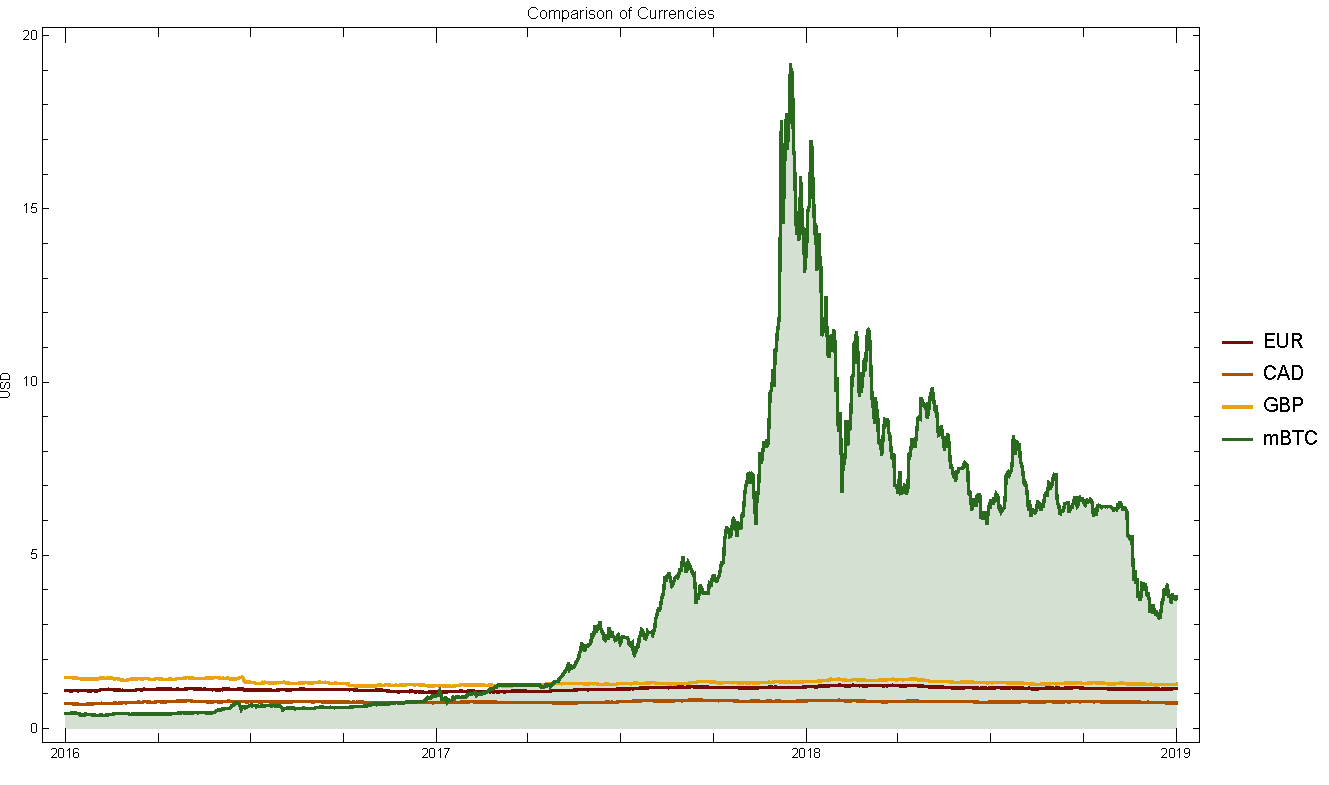
\includegraphics[width=0.5\textwidth]{figures/allCurrencies.pdf}
	\caption{\label{fig:btcandfiat}Comparison among fiat currencies and Bitcoin: The values are retrieved daily between  01 Jan 2016 and 01 Jan 2019. Note that 1000 mBTC = 1 BTC.}
\end{figure}
%========================%

From the inception of exchanges for buying and selling BTC for USD in 2010 to the time of writing, the exchange rate of BTC with the USD has been marked by extremely volatile with large fluctuations in its value that are atypical of a government-managed currency. Figure~\ref{fig:btcandfiat} illustrates this volatility by plotting the exchange rate of BTC (with the USD) alongside the same exchange rate for three economic zones---Europe, UK, and Canada---which all appear relatively stable. Note that Figure~\ref{fig:btcandfiat} deliberately includes the UK's referendum on exiting the EU (`Brexit') in June 2016, which was followed by a `sharp decline' and `volatility' in GBP's exchange rate.\footnote{Descriptions from the following \textit{BBC} articles: ``The markets facing trading turmoil'' (27 Jun 2016) and ``How does Brexit affect the pound?'' (15 Jan 2019).}  Relative to BTC however, this `severe swing' looks like a mild pinch of GBP's exchange rate with EUR in Figure~\ref{fig:btcandfiat}.

In response to Bitcoin's extreme volatility, a flood of proposals have been made for alternative designs that would offer a more stable exchange rate (called `stablecoins') between such a proposed stablecoin and a government-issued currency like the USD. Broadly, the proposals can be split into two categories: ones that essentially create a digital representation of a fiat currency that can be transacted like a cryptocurrency, and ones that propose separate currencies with some mechanism for stability and/or intervention built into the design.

\paragraph{Contributions.} This paper is essentially a survey of work on stablecoins but we aim at making a number of subtle research contributions to ensure this survey is useful to the reader. First and foremost, we are very selective in the concepts from finance we bring into the survey and explain each from first principles, while attempting to minimize or eliminate jargon. Next we distill stablecoin proposals down to a set of fundamental primitives and describe how these concepts work, as opposed to enumerating the intricate details of how a particular `brand' of stablecoins works today---details that could change tomorrow. We do provide, as the reader probably expects, a chart mapping existing stablecoin brands into our categorization. Additionally, we also consider the question and potential for the stability of index-cryptocurrencies (namely gas which is used in Ethereum), which are very pertinent to a discussion of stablecoins, yet not typically addressed. Last, we offer a novel visualization style for exchange rates we have not seen before used for exchange rates.

% Most of the coins are mostly focusing on the supporting infrastructure, maybe we also have to talk about the supporting infrastructure of the stablecoin


%========================%
\section{Related Work}
\label{sec:lit}

An early idea for a stable cryptocurrency was introduced by Ametrano in 2016~\cite{ametrano2016hayek} which tweaked supply (see Section~\ref{sec:stability}) In 2017, Robert Sams introduced a new dual token system that uses two coins to achieve price stability: (i) a stablecoin (\eg fiat currency) and (ii) a volatile coin (\eg equity shares)~\cite{sams2015note} (see Section~\ref{sec:stability}). These informed the designs of stablecoins we discuss in the paper.

There are many blog posts and professional reports providing an overview of stablecoins with essentially the same goal as this paper. Most have the same general categorization: (i) fiat-collateralized, (ii) crypto-collateralized and (iii) non-collateralized, also known as algorithmic,\eg~\cite{hackernoon, comprehensiveOverview, linkedin}. Buterin, in one of the earliest blog posts on stable cryptocurrencies, discussed different techniques to measure cryptocurrencies' price and how to make adjustments in the supply to achieve a fixed price accordingly~\cite{TheSearc7:online}. Bitmex looked at the mechanics of the distributed stablecoins while focusing on two case studies (\ie BitShares (BitUSD) and MakerDAO (Dai))~\cite{bitmex}. Another report by crypto company Blockchain provides an extensive classification of 57 stablecoins together with discussions on issues related to governance (\eg legal structure, investors, partners \etc)~\cite{reportone}. They extend this research in a newly published report that reflects a significant update on their previous work~\cite{reporttwo}. In one of its blog posts, Consensys \footnote{https://consensys.net} describes stablecoins as ``crypto-assets that maintain a stable value against a target price (\eg USD)'' and classify them according to three main categories~\cite{StateofS96:online}. In~\cite{cryptoinsider}, the authors use a slightly different categorization to group 13 stablecoin projects into two broad categories: (i) centralized-- which itself contains subcategories based on the type of the asset the coins are backed by (\eg fiat and gold), (ii) decentralized. Our survey can be differentiated from the related work in its focus: we strive for clear descriptions of the mechanics of stability within a coin, without glossing over details or substituting financial jargon for explanation. We focus less on any infrastructure around a stablecoin deployment (\eg it's code, interactions between contracts, governance, \etc).

%Cite Ross Anderson's paper :"Bitcoin Reducx" :
% Anderson\etal discuss different negative externalities that are introduced by Bitcoin~\cite{anderson2019bitcoin}. They perform and discuss taint tracking using First-In-First-Out (FIFO) algorithm ( inspired by the Clayton’s case) on some well-established Bitcoin theft scenarios. They also point out that crypto space needs effective regulation in order to function properly and securely, at the end they provide regulatory remarks for the future.


%========================%

\section{Preliminaries}

\subsection{Prices}

If 1 BTC is worth \$3598.76 USD, as Google says it is at the time of writing, what does that actually mean? There are several subtleties here: (1) what that price actually represents, (2) the relationship between a quoted price and its actual price, (3) the concept that prices are really an exchange of one type of valuable good for another, and (4) the distinction between something's price and its value. The quoted price means that two (hopefully different\footnote{A trade between the same person is called a wash trade and is illegal in most regulated markets.}) people recently exchanged BTC and USD at a valuation of 1 BTC for \$3598.76 USD. First, note that it does not necessarily mean that exactly 1 BTC was exchanged --- it could have been 1 mBTC for \$3.60 or 1000 BTC for \$36M USD. Further, this valuation on the previous trade does not mean you will necessarily be able to exchange 1 BTC for \$3598.76 USD. Last sale price is an indicator of current price that becomes stale as time between subsequent exchanges increase (for example, for a house that last sold 30 years ago, last sale price on a house is not a good indicator of current price).

Instead, we will use the idea of that a cryptocurrency (or any asset) has two prices: (1) the most someone is willing to pay and (2) the least someone is willing to sell for. These are referred to as the best bid price and best ask (or offer) price respectively. Note that the best bid price should logically be less than the best ask price, otherwise an exchange would happen (such prices might occasionally `cross' but this should be temporal and quickly resolved with an exchange). The spread between these prices is called the bid-ask spread.

To understand why this is relevant to stablecoins, consider an example. Say a stablecoin is designed to ensure one unit is always priced at \$1 USD. To argue stability, one must show both that (1) the bid price should never exceed \$1 dollar and (2) the offer price should never dip below \$1 USD. Note, conversely, that bids can dip below \$1 USD (everyone prefers to pay less than something is worth) and asks can exceed \$1 USD (everyone prefers to receive more than something is worth).

\subsection{Exchange Rates}

Consider that several hours after writing the previous section, 1 BTC is now priced at \$3566.56 USD. In one sense, the price of BTC decreased by \$32.20. However it is exactly equivalent to say the price of \$1 USD increased by 0.002 mBTC. This raises a natural question: did BTC decrease in price or did USD increase in price? With an exchange rate, it is impossible to tell. We only know that the price of BTC and USD became closer in price over this short period of time.

To determine which currency is moving, one might consider a third or forth currencies (\cf US Dollar Index) to try and triangulate if BTC is moving in price, or USD is moving in price, or both. For example, in Figure~\ref{fig:btcandfiat} it certainly appears that BTC is the currency that is moving because the rest of the currencies are stable relative to each other. The only alternative is that USD, EUR, GBP, and CAD are volatile currencies that move together as a cluster relative to the stability of BTC. But it is much simpler to conclude that BTC is moving.

%========================%
\begin{figure*}[t]
	\centering
	\subfloat[GBP with respect to EUR and USD.]{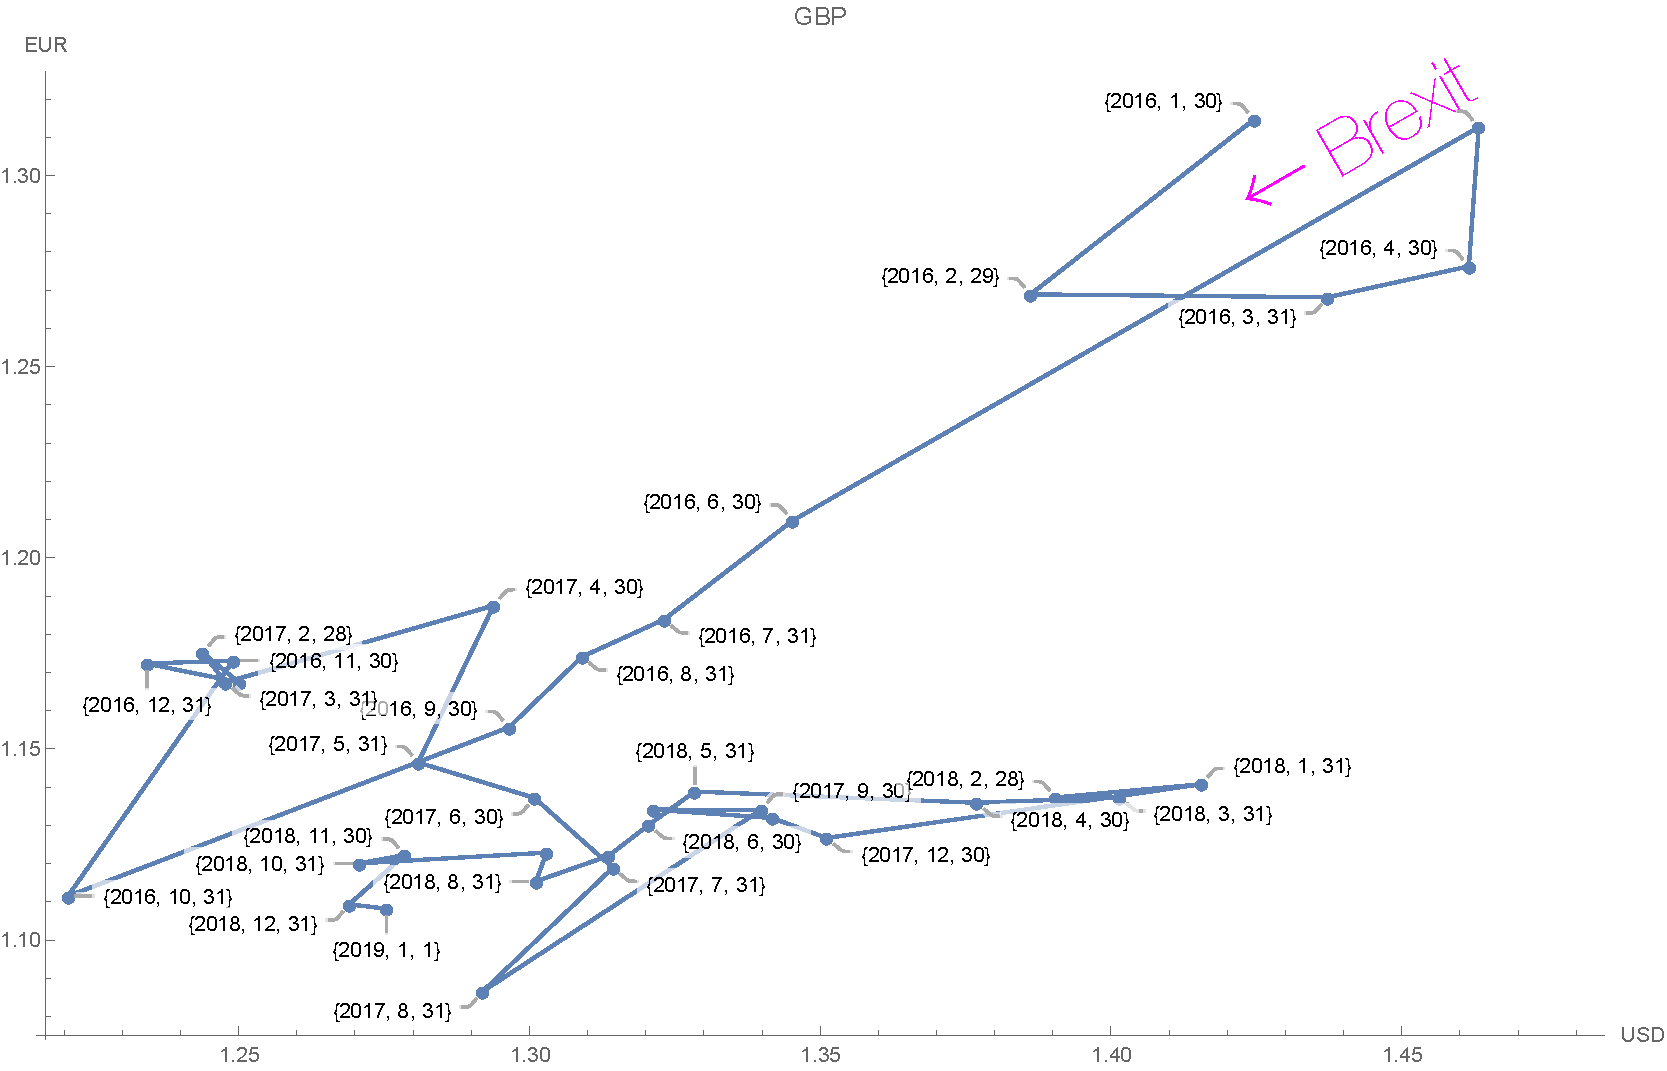
\includegraphics[width=0.65\textwidth]{figures/gbpBrexit.pdf}\label{fig:brexit}}
	\hfill
	\subfloat[Direction labels.]{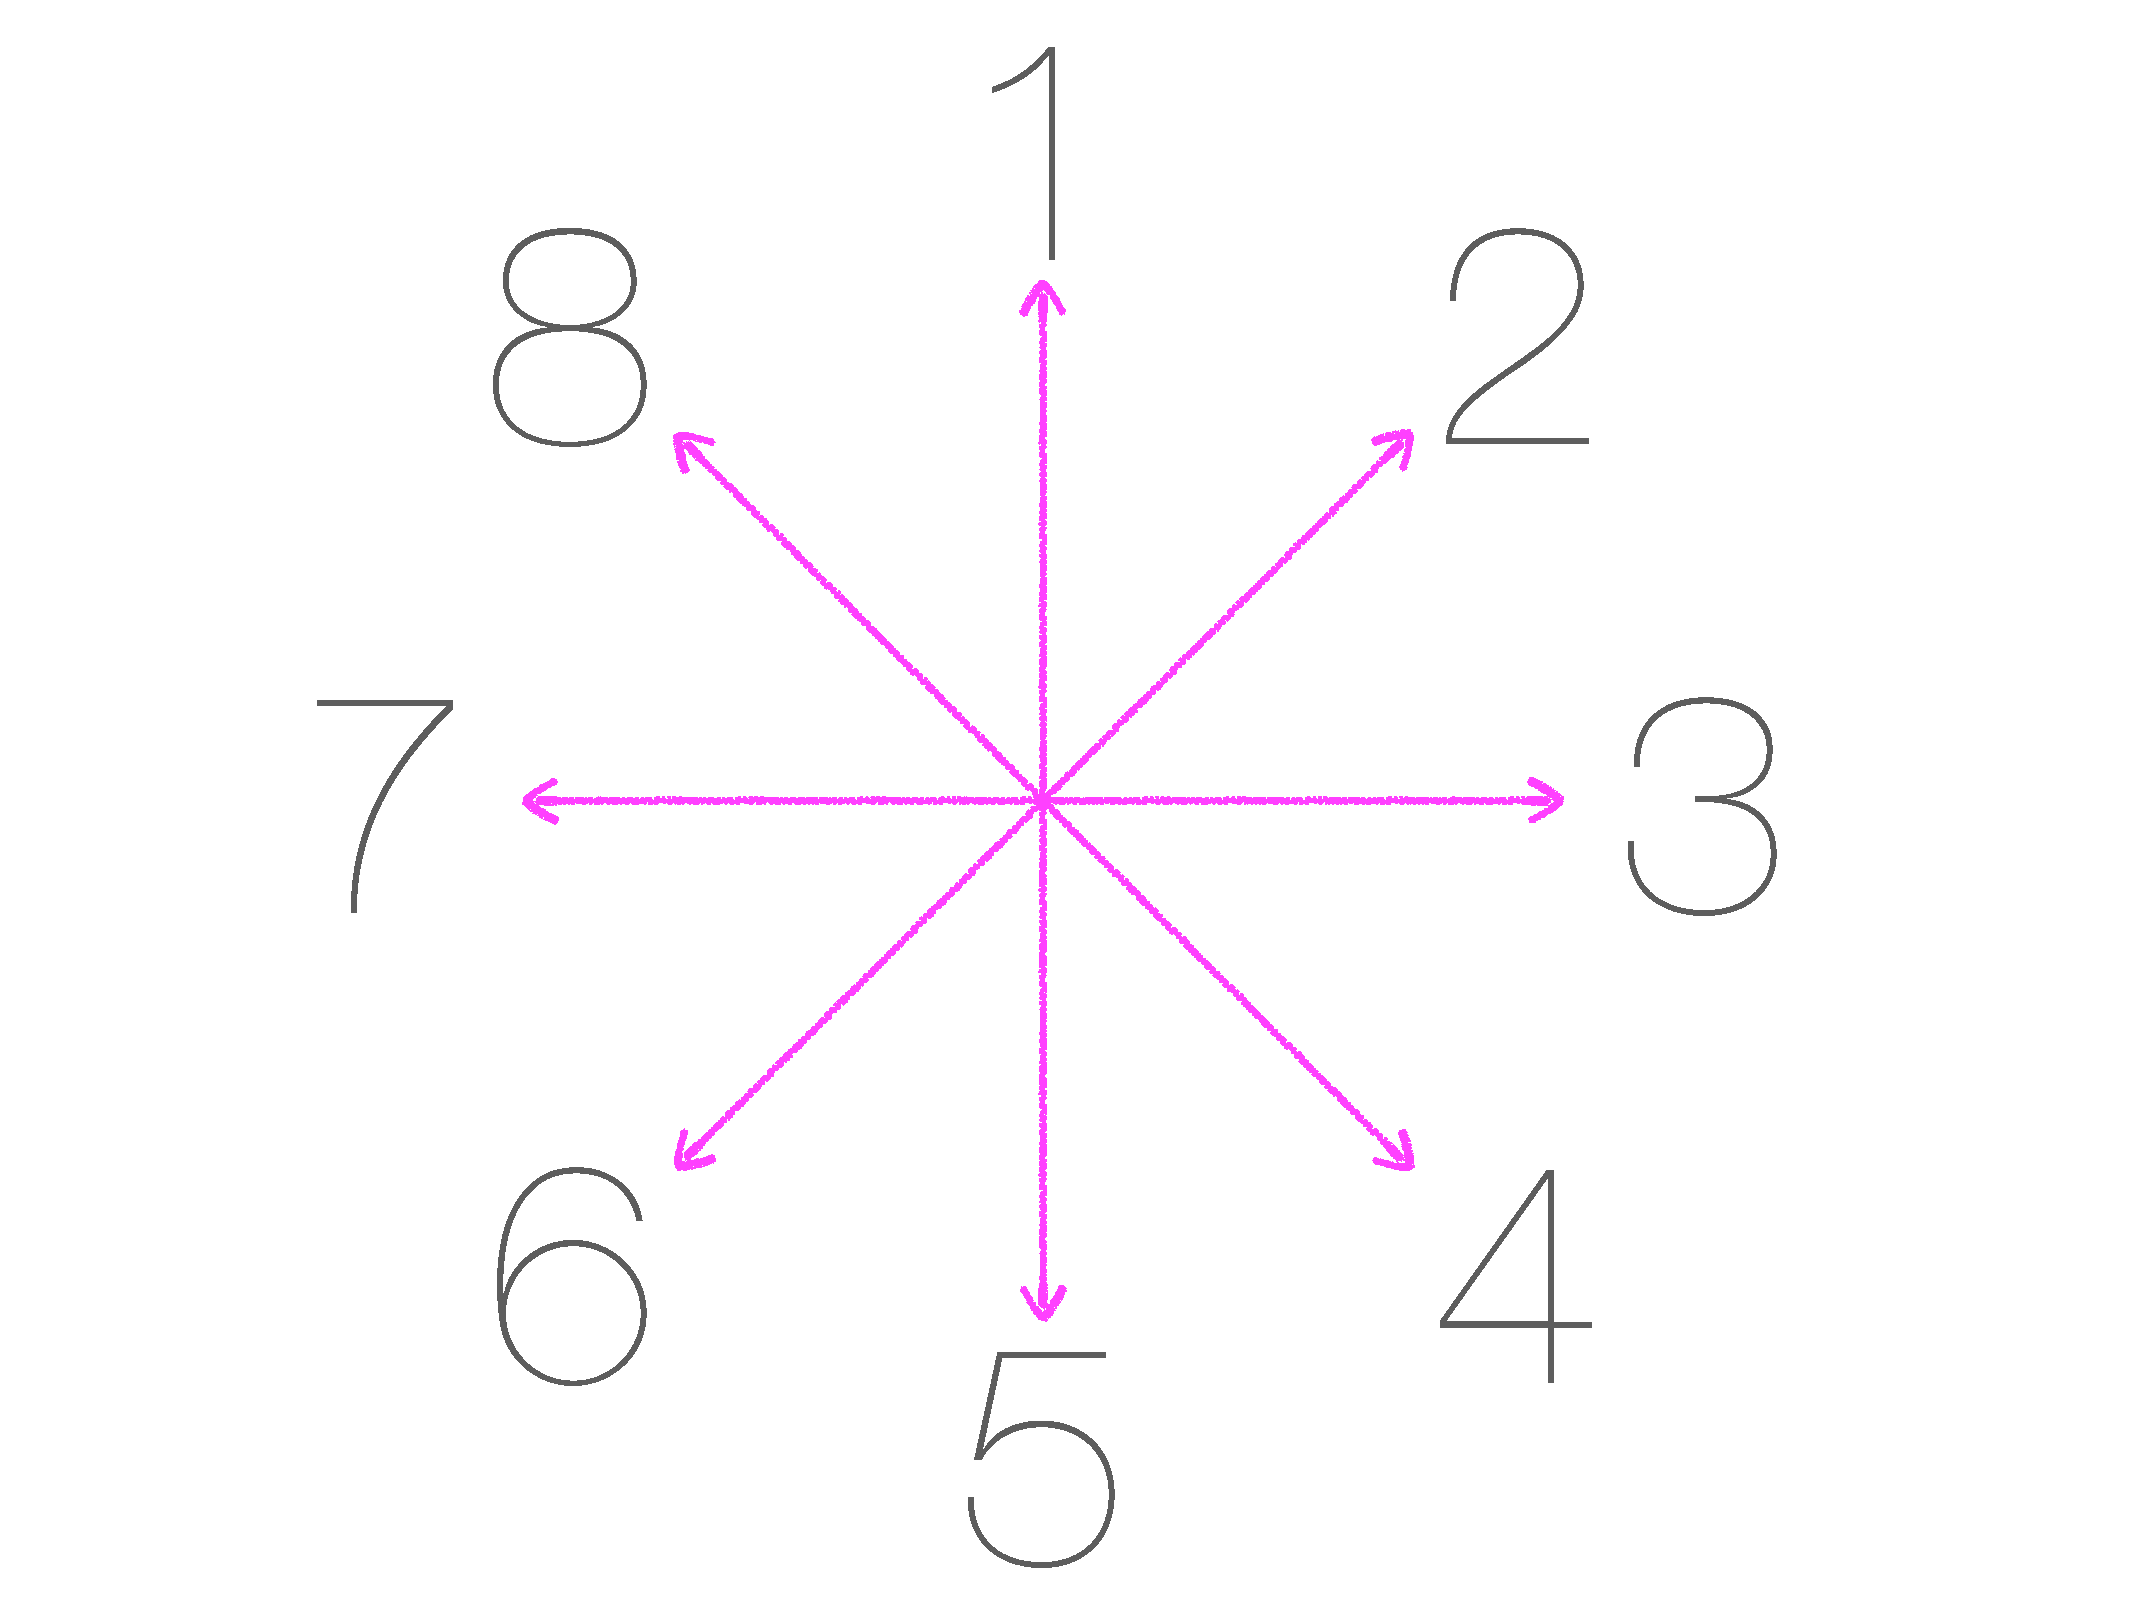
\includegraphics[width=0.25\textwidth]{figures/compass.pdf}\label{fig:legend}}
	\hfill
	\subfloat[The simpliest interpretation of the plots where $X$ refers to the currency on the x-axis (likewise $Y$).]{
	\begin{tabular}{|c|l|}
\hline
\textbf{Direction} & \textbf{Interpretation}   \\ \hline

         1/5                & $Y$ is losing (1) / gaining (5) value \\ \hline
         2/6                & Plotted asset is gaining (2) / losing (6) value \\ \hline
         3/7                & $X$ is losing (3) / gaining (7) value \\ \hline
         4/8                & \multicolumn{1}{p{13cm}|}{Plotted asset is gaining (4) / losing (8) value against $X$, while losing (4) / gaining (8) value against $Y$} \\ \hline

\end{tabular}
	}
	\caption{A connected scatter plot of GBP's exchange rate with EUR and USD demonstrating the effect of Brexit on GBP. Supporting documentation helps interpret the line movements in the plot.\label{fig:Comparison}}
\end{figure*}
%========================%

In order to apply this same logic in a visual way, we have created a number of charts like the one provided in Figure~\ref{fig:brexit}. Unlike most exchange rate graphs, these do not use a time axis. Instead each axis is a reference currency. In this case, the price of GBP (plotted value) in USD (x-axis) and EUR (y-axis) forms a coordinate. For the last day of each month, a new coordinate is added and joined with a line from the previous value. This is inspired by similar charts on the website FiveThiryEight for things like kicking distance in football\footnote{``The 52 Best---And Weirdest---Charts We Made In 2016,'' \textit{FiveThirtyEight}, 30 Dec 2016.} and they have been called connected scatter plots.

Lines in a connected scatter plot can move in any direction. Figure~\ref{fig:legend} shows how we number the directions from 1 (upward or due north) clockwise to 8 (north-west). For each direction, we describe the simplest interpretation of what that price direction means. By simplest, we mean specifically that we keep an explanation that involves a single currency moving rather than an explanation that involves a pair of currencies moving in tandem. For example, in Figure~\ref{fig:brexit}, GBP shows a drastic movement along direction 6 starting at the time period marked Brexit. This means that GBP is losing value against both EUR and USD. The simplest explanation is that the movements are originating from GBP which is consistent with it losing value after Brexit. Later, GBP shows a lot of horizontal movements along the 7/3 line. The simplest explanation for this segment is volatility in USD rather than GBP.
A copy of the datasets and codes of all the charts can be found on our GitHub repository. \footnote{https://github.com/ Removed for anonymity.}


We will return to these charts later in Section~\ref{sec:stability} where we will use a government currency as one reference (USD on the x-axis) and a cryptocurrency as the other reference (BTC on the y-axis). A stablecoin should exhibit mostly vertical movements along the 1/5 direction.

\subsection{Valuation}

Recall that in the previous section, 1 BTC was priced at \$3566.56 USD. This means that two people recently swapped some amount of BTC and USD for the stated valuation. Does this mean 1 BTC is worth \$3566.56 USD? Value can mean different things in different contexts. The market value of a currency does present one type of value --- its replacement value, or the cost in USD to replace it. Note that more technically, one should  determine replacement value from the set of best offer prices sufficient to cover the volume of BTC being valued.

But does this mean that BTC is fundamentally worth \$3566.56 USD. This is unlikely because by the time you read this paper, the price of BTC in USD is probably quite different from this quoted value (perhaps humorously so). So what constitutes fundamental value? And why do prices change over time?

Stocks, which represent ownership in a firm, and thus a stake in the firm's equity. Therefore shares (called equities) have a fundamental value called its book value: simplified, it is the firm's capital or equity (the value of its assets minus the value of its liabilities, as reported on its annual audited financial statement) divided by the number of outstanding shares. Working in reverse, the price of a single share multiplied by the number of shares represents the market capitalization of the firm. In theory, these numbers should be the same but often are not. When the market capitalization exceeds the reported capital, the market believes the firm's capital will increase over time. If the market capitalization is less than the reported capital, it demonstrates a lack of confidence in the soundness of the firm's financial statements. Floating currencies like the USD, EUR, GBP, and CAD do not have the equivalent of a book value.

To explain Bitcoin's exchange rate with fiat currencies, an oft-repeated theory has emerged that attributes Bitcoin's value to the hydro consumed by blockchain mining. While imprecise, the theory suggests that if a valuable resource $x$ is consumed to produce $y$, the value of $x$ is imparted into $y$. Setting aside the nuance that the hydro contributed to the Bitcoin system only indirectly produces new coins (it produces blocks, and blocks produce coins only for now), there is no economic principle underlying this transfer of value.



\subsection{Stability and Volatility}

When the price of a currency changes over time, it is due to one of two reasons: new information about the currency's fundamental value (even if we cannot concretely say what it is) or transitory volatility due to the trading activites of uninformed traders~\cite{harris2003trading}. For a government issued currencies, information like national inflation rates, macro-economic policies, changes in trade flows, and changes in capital flows seem predictive of changes in the value of the country's currency~\cite{harris2003trading}. Note that a cryptocurrency, like Bitcoin, has none of these indicators. While volatility can be measured mathematically (using variances or deviations), most stablecoins do not offer a concrete, positive definition of what stability means. They tend to be defined by a negative sentiment of what they do not want (the volatility of Bitcoin) rather than a positive sentiment of what they do want.

\subsection{Functions of Money}

There is controversy over whether Bitcoin, and other cryptocurrencies, can even be classified as currencies. The original intent from Bitcoin's creator was for it to be a currency, however it has been assigned many different classifications: from a digitally scarce commodity, to a speculative instrument, to an entirely new asset class.

Most introductory finance textbooks classify currencies according to a set of three core properties it should fulfill for its users. It should operate as a medium of exchange, which roughly means that Alice will accept the currency from Bob because she is confident Carol will later accept it from her. Given the existence of exchange services, Bitcoin is generally considered an acceptable medium of exchange (albeit with some friction). Next, a currency is useful when it serves as the unit of account for pricing other assets. Bitcoin is almost never used as a unit of account and if goods are sold for Bitcoin, it is often priced in, say, USD with a short-lived (\eg 2 minute) spot conversion of the price to BTC for Bitcoin purchases. Finally, currencies should represent a stable store of value. Alice will not accept a currency that depreciates quickly in value from Bob because even though Carol might accept it, what she can obtain from Carol in exchange will be worth less. Less intuitively, currencies that appreciate quickly in value are equally problematic. Alice might gladly accept it from Bob but Bob is unlikely to part with it, and so currencies like this tend to be hoarded. They also hamper lending (see next section).

The goal of a stablecoin is to add the store of value feature to cryptocurrencies, which are already a somewhat adequate medium of exchange. Further, if the currency is stable, it may become a more prominent to use it as a unit of account. Thus stablecoins are intended to make cryptocurrencies more currency-like.~\cite{rogoff2017curse}

 %Cite Curse of Cash: Is its cited in the right place? (above parag)

\subsection{Lending}

Lending a volatile currency poses a risk for both the cash provider and cash taker. Currency depreciation results in the cash provider being repaid less than what they initially provided, and currency appreciation results in the cash taker having to repay a great amount than what was borrowed. Thus a stable currency enables low-risk lending which is beneficial to all participants and is the cornerstone of a modern economy. Okoye \etal put it in a way that is hard to improve on:

\begin{quote}

``It is difficult to overstate the role of lending in a modern economy. Take, as an illustrative example, the role of a central bank; one of the main national institutes (along with the treasury) that cryptocurrencies aim to displace. First and foremost, a central bank is an actual bank, providing accounts for its member banks to deposit money and earn interest. Member banks provide interest-earning accounts to the public. Interest is paid to the public because banks use the deposited money to form loans. Because central bank interest rates are low, banks prefer to lend to other banks any excess cash they hold at day's end instead of depositing them (other banks borrow to meet liquidity requirements). These loans earn interest, and central banks target this specific lending rate when they intervene in the economy. The most common intervention is the buying (circulating new money) or selling (removing circulating money) of government bonds, which are interest-earning loans from investors to the government. Central banks will also provide loans (of `last resort') to banks unable to secure loans from other banks, typically during some sort of liquidity crisis. An economy without loans would have no interest rates, no bonds, and essentially nothing for a modern central bank to do.~\cite{okoyetoward}''

\end{quote}






% = = = = = = = = = = = = = = = = = = = = = = = = = = = = = = = = %

\section{Type 1: Backed Stablecoins}
\label{sec:t1}

In this section, we discuss the first type of stablecoin. These coins try to directly match the stability of a second asset, such as the USD. These coins could not exist without their target asset. In Section~\ref{sec:t2}, we consider the second type of coin which is a standalone currency that use intervention (algorithmic and/or human) to reduce volatility.

% !TEX root = ../main.tex


%-------------------Fancy Table ----------------------%

% = = = Rotated Table Entry \headrow


\newcommand{\headrow}[1]{\multicolumn{1}{c}{\adjustbox{angle=65,lap=\width-0.5em}{#1}}}

% = = = Table bullets: \full and \prt (full and part)

\newcommand{\full}{$\bullet$}
\newcommand{\prt}{$\circ$}
% ------------------------------------------------------------------------------------------------------------------------------------------------%
%Stablecoin projects%

\definecolor{UnitedNationBlue}{rgb}{0.30,0.53,1}
\definecolor{LightSteelBlue}{rgb}{0.69,0.77,0.87}
\definecolor{LightGrey}{rgb}{0.83,0.83,0.83}


\begin{table*}[t]
\centering

\begin{tabular}{|l|l|l|l|l|}

\hline
\rowcolor{lightgray}
\textbf{Class} & \textbf{Mechanism} & \textbf{Resembles} & Rank \\  \hline
% = = = = = = = = = = = = = = = = = = = = = = = = = = = = = = = = = = = = = = = = = = = = = = = = = = = = = = = = = = = = = = = = = = = = = = %
\multirow{17}{*}{Backed}		
						& \multirow{8}{*}{Directly-Backed \& Redeemable$^{\dagger}$}	& USDC 			& 20 \\ \cline{3-4}
						&													& TrueUSD 		& 26 \\ \cline{3-4}	
						&													& Paxos 			& 38 \\ \cline{3-4}		
						&													& Gemini Dollar 	& 52 \\ \cline{3-4}
						&													& StableUSD (USDS) & 685 \\ \cline{3-4}
						&													& Stronghold USD 	& 891 \\ \cline{3-4}
						&													& Petro 			& 1210 \\ \cline{3-4}
						&	& \multicolumn{1}{p{5cm}|}{Ekon, WBTC, emparta} & $\perp$ \\ \cline{2-4}
% = = = = = = = = = = = = = = = = = = = = = = = = = = = = = = = = = = = = = = = = = = = = = = = = = = = = = = = = = = = = = = = = = = = = = = %
						& \multirow{6}{*}{Directly-Backed}  							& Tether 			& 6 \\ \cline{3-4}
						&													& EURSToken 		& 95 \\ \cline{3-4}
						&													& BitCNY 			& 304 \\ \cline{3-4}
						&													& Terracoin 		& 1280 \\ \cline{3-4}
						&													& Saga 			& 1495 \\  \cline{3-4}
						&	& \multicolumn{1}{p{5cm}|}{GJY, Novatti AUD, UPUSD} & $\perp$ \\ \cline{2-4} 						
% = = = = = = = = = = = = = = = = = = = = = = = = = = = = = = = = = = = = = = = = = = = = = = = = = = = = = = = = = = = = = = = = = = = = = = %
						& \multirow{3}{*}{Indirectly-Backed}							& Dai 			& 57 \\ \cline{3-4}
                                                &													& BitUSD 			& 398 \\  \cline{3-4}
                                                & 													& Nomin			& $\perp$ \\ \cline{1-4}
% = = = = = = = = = = = = = = = = = = = = = = = = = = = = = = = = = = = = = = = = = = = = = = = = = = = = = = = = = = = = = = = = = = = = = = %
%						& \multirow{1}{*}{Market Manipulation} 						& NuBits			& 892 \\ \cline{1-4}
\multirow{5}{*}{Intervention}                                                           

% = = = = = = = = = = = = = = = = = = = = = = = = = = = = = = = = = = = = = = = = = = = = = = = = = = = = = = = = = = = = = = = = = = = = = = %
						& \multirow{2}{*}{Money Supply Adjustments}  				& Ampleforth		& $\perp$  \\ \cline{3-4}
						&   													& RSCoin 			& $\perp$  \\ \cline{2-4}
% = = = = = = = = = = = = = = = = = = = = = = = = = = = = = = = = = = = = = = = = = = = = = = = = = = = = = = = = = = = = = = = = = = = = = = %
						& \multirow{2}{*}{Asset Transfer}  							& NuBits			& 892 \\ \cline{3-4}
						&													& CarbonUSD		& 1262 \\ \cline{3-4}
						&													& Basecoin 		& $\perp$ \\ \cline{1-4}
% = = = = = = = = = = = = = = = = = = = = = = = = = = = = = = = = = = = = = = = = = = = = = = = = = = = = = = = = = = = = = = = = = = = = = = %
%						& \multirow{2}{*}{TBD: Internal }  								& Nautiluscoin 		& $\perp$ \\ \cline{3-4}
% = = = = = = = = = = = = = = = = = = = = = = = = = = = = = = = = = = = = = = = = = = = = = = = = = = = = = = = = = = = = = = = = = = = = = = %
\hline
\end{tabular}
\caption{Stablecoin proposals as of January 11, 2019. $\dagger$ \textit{Disclaimer:} Projects are classified according to what they assert; \eg we provide no warranty that projects classified as `redeemable' provide actual redemption of the assets that back their coins. Rank corresponds to \textit{CoinMarketCap}.\label{tab:stablecoins}}
\end{table*}
% ------------------------------------------------------------------------------------------------------------------------------------------------%





In Table~\ref{tab:stablecoins}, we show the taxonomy we use to classify stablecoins. As mentioned earlier in related work (see Section~\ref{sec:lit}), taxonomies for stablecoins have been proposed many times. The focus of our taxonomy is a bit different. We do not care about classification \textit{per se}---we view our work as a tutorial on how to build a stablecoin, and the taxonomy are simply is a set of directions a designer can choose between or combine. They are based on proposals for stablecons, as well as insights from monetary policy for governmental currencies.

To find stablecoin projects, we performed a number of search queries on \textit{CoinDesk}, an online news source for cryptocurrencies and blockchain technology.\footnote{https://www.coindesk.com/} Our search terms included ``stablecoins,'' ``stability,'' and ``price-stable.'' We read 185 articles up to January 11, 2019 and extracted the names of projects. For the 25 projects for which we could find sufficient documentation, we classified them in Table~\ref{tab:stablecoins}. This classification is done according to what the projects assert they do---we provide no warranty of what the projects do in reality. Finally, within each category, we sort projects according to their rank on \textit{CoinMarketCap} which ranks cryptocurrencies that are actively traded on an exchange service.\footnote{https://coinmarketcap.com} Unlisted projects are ranked $\perp$.

% = = = = = = = = = = = = = = = = = = = = = = = = = = = = = = = = %

\begin{table*}[t!]
\centering
\begin{tabular}{|l|}
\multicolumn{1}{c}{\textbf{Stability Mechanisms}}  \\ \hline

\multicolumn{1}{|p{\textwidth}|}{\textbf{Directly Backed and Redeemable.}\newline \footnotesize Alice is a trusted third party and uses Ethereum to instantiate a decentralized application (DApp) which issues 1000 AliceCoins as standard tokens (\eg ERC20). She asks \$1 USD for 1 AliceCoin and promises to redeem any AliceCoin for \$1 USD. If Bob buys 10 AliceCoins for \$10 USD, Alice deposits the \$10 USD in a bank account. Any time Alice receives a buy order for AliceCoins and does not have any left to sell, she creates new ones to sell. If Carol wants to redeem 5 AliceCoins, Alice withdraws \$5 USD and exchanges it with Carol, taking those AliceCoins out of circulation. Alice frequently publishes bank statements showing that her account holds enough USD to redeem all coins in circulation (the number of AliceCoins can be checked anytime on Ethereum).} \\ \hline

\multicolumn{1}{|p{\textwidth}|}{\textbf{Directly Backed.} \newline \footnotesize  Again, Alice is a trusted third party that issues 1000 AliceCoins as ERC20 tokens. She asks \$1 USD for 1 AliceCoin and promises to deposit and hold the payment in a bank account. As before, Alice creates new AliceCoins when she runs out and publishes frequent bank statements. Unlike above, she offers no direct redemption of AliceCoins for USD.} \\ \hline

\multicolumn{1}{|p{\textwidth}|}{\textbf{Indirectly Backed.} \newline \footnotesize Alice is no longer assumed to be trustworthy. She sets up a DApp that can hold ETH and issue tokens. The DApp determines how much ETH is equivalent to \$1.50 USD using the current exchange rate, provided to the DApp by a trusted third party oracle, and Alice deposits this amount of ETH into the DApp. The DApp issues to Alice two places in a line --- each place is a transferrable token. At some future time, the holder of the first place in line can redeem up to \$1.00 USD worth of the deposited ETH at the future exchange rate, and the holder of the second place in line gets any remaining ETH. Alice will transfer the first place in line (as a stable coin called AliceCoin) to Bob for \$1.00 USD, and will hold or sell the second place in line. When Bob redeems the AliceCoin, it will be worth \$1 USD in ETH when the entire deposit of ETH is worth more than \$1 USD. If the exchange rate drops enough, the deposit will be worth less than \$1 USD --- Bob will get all of the deposit and the holder of the second place in line will get nothing.} \\ \hline

\multicolumn{1}{|p{\textwidth}|}{\textbf{Money Supply Adjustments.} \newline \footnotesize Alice forks Bitcoin to create a new altcoin called AliceCoin. She tweaks the schedule for releasing new AliceCoins (called the coinbase amount in Bitcoin) according to the rules outlined below. She sets up a trusted oracle for the latest exchange rate of AliceCoins to USD. AliceCoin is programmed to apply an intervention when the price of an AliceCoin exceeds \$1.02 USD or dips below \$0.98 USD. If the price exceeds \$1.02 USD, the miner is allowed to increase the coinbase amount (the amount is determined by some mathematical relationship with how much the price exceeds \$1.02 USD). If the price dips under \$0.98 USD, the miner must decrease the coinbase amount based on the same relationship. The correctness of the claimed coinbase is verified by other miners in deciding to accept or reject a mined block, as per all other checked conditions in Bitcoin.} \\ \hline

\multicolumn{1}{|p{\textwidth}|}{\textbf{Asset Transfer.} \newline \footnotesize Alice instantiates a DApp with an ERC20 token called AliceCoin. The DApp is programmed to apply an intervention when the price of an AliceCoin exceeds \$1.02 USD or dips below \$0.98 USD according to a trusted oracle. If the price exceeds \$1.02 USD, the DApp creates new a set of AliceCoins (as above, according to some mathematical relationship) and transfers them to users waiting in line for them. How do users wait in line? When the price dips under \$0.98 USD, the DApp creates new positions at the end of the line and auctions them off to the highest bidder. The payment for a place in line is made in AliceCoins from the bidder to the DApp and the DApp destroys the payment. The place in line is a transferrable token. If the line is empty, AliceCoins are distributed according to a fallback policy (see main text).} \\ \hline

\end{tabular}
\caption{Major types of stability mechanisms for stablecoins.\label{tab:mech}}
\end{table*}

% = = = = = = = = = = = = = = = = = = = = = = = = = = = = = = = = %

\subsection{Directly-Backed and Redeemable}
\label{sec:redeem}

The first direction one might take in producing a stablecoin is the creation of a digital representation (or tokenization) of a fiat currency, commodity, or portfolio of assets. Tokens are designed to have the same price (and thus volatility) as the underlying portfolio. To further enable an equivalence of value (we will explain how shortly), the digital token can be redeemed on-demand for the underlying asset. For simplicity, we will consider a cryptocurrency designed to digitally represent the USD.

The idea of tokenizing USD (or EUR or gold) for use on the internet is not new. Liberty Reserve and e-gold provided a similar service. Liberty Reserve dollars were redeemable in principle, but only indirectly through an intermediary and redemption could be refused. Meanwhile, e-gold was not redeemable (see next section of a discussion of the consequences of this). What is novel about a stable cryptocurrency is that transactions are not done on a centralized server, but rather finalized and settled on a decentralized blockchain. However since directly-backed stablecoins reintroduce centralization to create the digital tokens, maintain reserves of the underlying asset, and process redemption requests, the benefit of a decentralized transaction platform is marginal.

\paragraph{Process.} See Table~\ref{tab:mech}.

\paragraph{Price Stability.} For simplicity, assume all transactions are free and frictionless. Consider a bid for 1 AliceCoin that is greater than \$1 USD. Bob will sell an AliceCoin immediately for this price and will ask Alice to generate a new AliceCoin, deposit only \$1 USD for this, and keep the rest of the bid value as profit. Therefore bids in excess of \$1 USD will be temporal assuming Alice is quick to generate new coins on demand. Next, consider an ask for 1 AliceCoin for less than \$1 USD. Bob will immediately purchase this AliceCoin for its asking price, try to redeem it for \$1 USD from Alice, and if successful, keep the difference as profit. Bob's willingness is proportional to the expectation that it can actually be redeemed for \$1 USD. For an example, if he only buys at \$ 0.60 USD, it might reveal that Bob believes there is only a 60\% chance of redeeming the coin or that he can only redeem 60\% of its redemption value (the asker thinks it must be less, otherwise she'd rather redeem it than sell it).

Conclusion: the bid-ask spread will saddle \$1 USD and trades should execute close to \$1 USD assuming the market is close to 100\% confident in a frictionless creation and redemption process for of coins. In reality, fees and time delays for moving stablecoins and fiat payments will cause distortions.

\paragraph{Discussion.} Blockchain-based cryptocurrencies are designed to minimize trust in third parties. The trust assumption on stablecoins in this category are close to pre-blockchain currencies like Liberty Reserve and e-gold, who would maintain transaction details and account balances on a private server. Blockchain enables decentralized trust for the transactions, although it also makes them transparent---at least, as transparent as token movements are for the underlying contract and/or blockchain. This includes transactions with other decentralized applications. However the coin creation and redemption processes rely on trust.

A financial audit is an important step than can establish confidence in the redemption process, which in turns provides stable prices on coins being offered for sale. The auditor becomes a further trusted entity, and ties its reputation to the firm operating the stablecoin. For regulatory reasons, reputable auditing firms will want a clear indication of the coin's legality, as well as confidence in the firm's internal controls over the issuance and redemption of tokens and the custodianship of the backing assets. A sensible template for a stablecoins of this type will consist of three trusted entities: the firm operating the coin, a reputable auditor, and a reputable custodian of the assets.

If the firm operates in a jurisdiction with modern securities laws, the issuance of the stablecoins is likely subject to regulatory approval. Further, the redemption of the coins will serve as a main point of regulation, requiring financial reporting to prevent the kind of crime that was prevalent on pre-blockchain coins like Liberty Reserve and e-gold. A number of existing coins with operations in the United States have been reported as disallowing redemption for some holders.

% According to the recent blogpost in  (https://www.coindesk.com/winklevoss-crypto-gemini-gusd-stablecoin-redemption) Gemini has closed the account of some users and in some cases do not let redemption (some KYC issues) +     Paxos has has the same issue, although they let the user redeem their assets and then closed their account (https://www.ccn.com/paxos-standard-hassling-ethereum-traders-trying-to-redeem-stablecoin-pax-for-dollars)

A variety of firms and projects providing stablecoins in this category exist. Why so many? The differentiation between coins is along a few parameters: (1) the type of asset that can be redeemed for the coin: USD, EUR, gold, \etc; (2) the underlying blockchain (\eg Bitcoin, Ethereum, \etc) and the low-level technical design (updatable contracts, governance, \etc) ~\cite{geminido29:online}; and (3) the degree of regulatory compliance: paving forward in a highly regulated environment to bootstrap trust, or seeking under-regulated environments to move to market quickly and avoid government surveillance for participants.

% = = = = = = = = = = = = = = = = = = = = = = = = = = = = = = = = %

\subsection{Directly-Backed}
\label{sec:tether}

Next we consider stablecoins that are directly-backed---exactly as in the previous section but they do not offer a redemption process for the coin's underlying assets. Redemption is logistically complicated. Consider a USD-backed dollar---it is usually easier for a firm to receive USD payments from users than it is for it to send payments back, and sending payments opens up new exposure to regulation. Instead the firms behind these coins  pledge to keep the backing assets in trust for the duration of the circulating coins. We will shortly explain what impact there is on the exchange rate if it does not provide redemption---obviously, if redemption was inconsequential than no one would offer it as it increases costs and complexity. For our ranking in Table~\ref{tab:stablecoins}, if we could not find a clear assertion of redemption, we listed the project under this category.

\paragraph{Process.} See Table~\ref{tab:mech}.

\paragraph{Price Stability.} Again, assume all transactions are free and frictionless. Bids will not exceed \$1 for the same reason the coins in the previous section (Section~\ref{sec:redeem}). Consider an ask for 1 AliceCoin for less than \$1 USD. Bob will only immediately purchase this AliceCoin for its asking price if he has some assurance it will return to \$1 USD. Because it is not redeemable, the only mechanism that will push the value up is psychological: others in the market will ask \$1 USD because they believe it is valued at \$1 USD because it is backed by \$1 USD.

Conclusion: bids will not exceed \$1 USD but the best ask could vary from \$0 USD to \$1 USD without being immediately traded.

\paragraph{Discussion.} The idea of tokenizing assets and re-selling them in a useful format (\eg as a portfolio or in a way that is digitally compliant with standard trading software and automated accounting systems) is commonplace for standard financial assets, however most tokenizations of this type have some direct or indirect redeemable value. Consider two contrasting examples: a typical ETF and a typical trust fund. An electronically traded fund (ETF) will typically sell shares of a portfolio of assets, be redeemable for the assets on-demand, and will be priced closely ($\pm 1\%$) to the value of its underlying assets---it is most like the stablecoins in Section~\ref{sec:redeem}. A simplification of a (close-ended) trust fund is as follows: a firm will set up a special corporation to hold the assets, the tokens are not directly redeemable, however the tokens are ownership shares in the special corporation---by owning the corporation, you effectively own its assets. Such a fund will trade with greater deviation from the value of its assets ($\pm 5\%$).

%There is middle category of redeemability.
%similar to indirect owership of gold. It is redeemable for a share of the company that holds the gold.
%check the backed ones for having shares or not

A coin that has no redemption, direct or indirect, will not clearly trade for a particular amount. An informal argument in favour of it being stable is that minting the coin is costly---it requires obtaining USD to hold in reserve. This feature serves an important function, albeit a different one. This bounds the firm from over-issuing tokens, which would cause the coin to loose value, however it does not ensure asks do not drop below \$1 USD.

The difference between the market value of a newly minted coin and the cost to produce it is called seignorage. A backed stablecoin has no seignorage: it sells for \$1 USD and requires holding \$1 USD to `produce' it. There appears to be a folk theorem that if minting asset X requires consuming asset Y, asset X will take on the value of asset Y (otherwise, who would produce X?). In reality, resources can be consumed to produce something of no value---that value is simply lost. A canvas that has been applied with acrylic paint might cost \$100 USD in raw materials; its value could none-the-less be much less than \$100 USD\ldots or much more.

%If Alice goes to Peter Luger's in Brooklyn, consumes a \$100 ribeye, and mints a literal shitcoin out of the result --- is that coin worth \$100 because it is ``backed'' by \$100 worth of steak?

Even if the market does not accept the psychology that a coin backed by \$1 USD should be priced at \$1 USD, it is still important to establish that the coin is actually backed as a guard against over-issuance. As in the previous section, holders of the coin will want assurance that the custodianship of the backing asset is sound. A financial audit by reputable firm is one method to provide this assurance. %\textblue{Recap: Is bitcoin really un-tethered?~\cite{griffin2018bitcoin}}.

%Tether attacks.

%There are discussions about whether Tether has an effect on Bitcoin's price~\cite{griffin2018bitcoin}. When there is a decrease in price, Tether is converted into Bitcoin and Bitcoin is sold for USD, when the prices increase. Then, that amount of USD is used to back Tether. 

%It seems like the issuance of new Tether, probably unbacked at that time, inflates the BTC price and then this is used as an advantage to back the issued tokens by selling BTC.

% TETHER: Does it artificially inflate BTC price? Do they issue un-backed tokens to reinforce BTC price, then sell BTC to fully back tokens?
%TETHER ATTACK: On October 15, 2018, tether, the market dominating stablecoin with a market cap of $2 billion, was attacked, breaking tether’s peg to USD, dropping its value by 7 percent but simultaneously driving up bitcoin and the whole crypto market by more than 10 percent.
%on October 15, 2018; where the price drastically surged from $6,376 at 12.31 UTC to $7,083 at 14.50 UTC. A downturn in price was seen approximately one hour after that to $6,821, before went stable at around $6,400 — $6,600. It was one of the one of the most unexpected fluctuations after a while. The first ‘stable coin’ tether (USDT) which supposedly pegged 1:1 to the U.S. dollar fell up to 15% at the same time as the price of bitcoin fluctuate wildly. The movement caused a loss of trust among traders, causing them to sell tether and invest in other cryptocurrencies. A massive selloff for tether against bitcoin was seen, resulting in a price rise in bitcoin.
%bitcoin and other crypto assets are perfectly negatively correlated with stablecoins.
%speculative attack


% = = = = = = = = = = = = = = = = = = = = = = = = = = = = = = = = %

\subsection{Indirectly-Backed}
\label{sec:dai}

The previous two sections describe coins that require a trusted firm to hold assets. The difference between these coins and traditional digital currencies like Liberty Reserve and e-gold is marginal---it is only that transactions are now decentralized. By contrasts, coins in this class prioritize decentralization and offer stablecoins that are issued, transacted, and redeemed in an autonomous fashion, while still being redeemable for USD. However these requirements are in conflict as there are no USD on a blockchain like Ethereum.

Coins in this section try to find a middle-ground. They introduce a single trusted element: an exchange rate of the underlying (non-stable) cryptocurrency on the blockchain (\eg ether) and a stable fiat currency (\eg USD). Since the blockchain has no inherent knowledge of the USD/ETH exchange rate, the rate is stored and periodically updated by a trusted entity called an oracle (the consensus of multiple oracles can also be referenced), and such a service could have useful applications beyond stablecoins.

Tokens then created when the equivalent of \$1 USD in ETH is collected, and redeemable for the equivalent of \$1 USD in ETH. Thus the amount of redeemable ETH can grow or shrink as the exchange rate with the USD changes. If it shrinks, the contract that issued the coin holds the difference and returns it to creator of the coin. If it grows, it is problematic because the contract cannot hold an unbounded amount of ETH. Thus the contract collects more than \$1 USD (say \$1.5 USD) when it mints a new coin to provide a buffer against falling ETH prices.

\paragraph{Process.} See Table~\ref{tab:mech}.

\paragraph{Price Stability.} Consider a bid for 1 AliceCoin that is greater than \$1 USD. Bob will sell an AliceCoin immediately for this price and will ask Alice to generate a new AliceCoin, pay her only \$1 USD for this, and keep the rest of the bid value as profit. (More generally, Bob could issue a BobCoin assuming the bid is for any coin backed by this type of contract). Therefore bids in excess of \$1 USD will be fulfilled as long as there are individuals willing to lock up a deposit of ETH that is 1.5x the face-value of what they receive. If there is a shortage of ETH for this purpose, AliceCoins might trade in excess of \$1 USD. It is important to note if Alice underwrites one of these contracts, retains the USD she sells the AliceCoin for, and the ETH/USD exchange rate changes, she will make or lose exactly the same amount of money as she would by simply holding the same amount of ETH she deposited. The exception is if the contract's deposit becomes worth less than the amount that can be redeemed from it --- in this case, Alice loses less money by underwriting the contract (the holder of the coin bears the loss) than if she held ETH.

% Case study?

Next, consider an ask for 1 AliceCoin less than \$1 USD. If the contract backing the coin has an ETH deposit valued at the bid price or more, Bob will immediately purchase the AliceCoin, redeem it for \$1 USD, and keep the difference as profit. If the contract's deposit is worth less than the bid price, the ask will not necessarily be filled. Therefore AliceCoins will trade for less \$1 USD when contracts have insufficient deposits, as might happen following a fast deterioration in the value of ETH relative to USD.

Conclusion: Indirectly-backed coins will fulfill bids greater than \$1 USD assuming there is a willingness for ETH holders to lock up their ETH. Asks less than \$1 USD for an indirectly-backed coin will also be quickly fulfilled when the exchange rate of ETH is favourable (by any amount) or when it decreases by a moderate amount. Asks less than \$1 USD will persist if ETH decreases substantially.

\paragraph{Discussion.} In standard finance, brokerages will lend money to investors but are concerned about getting it back in the case that the investors lose their borrowed money. They generally will require a deposit from the investor, monitor the investor's profits and losses, and liquidate the investor's position if their losses approach the deposited amount (or ask the investor to deposit more). This is premised on the assumption that prices do not fall too quickly to react and that the position can be sold quickly at a good price. Therefore it is a precedented premise that an indirectly-backed stablecoin can be redeemed quickly before the deposit is worth less than the coins, however ETH may be far more volatile than other financial instruments.

There are many design decisions to consider when deploying an indirectly-backed stablecoin: the ratio by which the initial deposit exceeds the redemption value (\eg 1.5x), if coins can be redeemed any time, if a third-party can trigger a redemption (\eg for a fee) if they notice a deposit is close to losing more value than the face value of the coins (before the coin holder does), how close the deposit can get to losing value before such a trigger, and if all deposits backing all such coins should be pooled together, so all coins are interchangeable (`fungible'), or each coin is tied to a specific deposit. Note that while allowing third parties to trigger a redemption seems like a sensible service, if the coin holder is not monitoring the situation, they will end up holding ETH, instead of an AliceCoin, which is still losing value. This mechanism is really only about maintaining the reputation of the stablecoin.

If the contract holding the deposit is thought of as a financial instrument (and the stablecoin could enable it to be sold from Alice to Bob), it appears to be a novel configuration. It however has certain aspects in common with existing financial instruments. We outline a few here for readers familiar with finance, but the rest of this section can otherwise be skipped. Repurchase agreements also over-collateralize to insure against a decrease in the collateralized asset's value. If the contracts are sold, the value depends on the future exchange rate and thus are effectively an ETH-settled derivative, but not of a standard type. Another way to think about the stablecoin and underlying contract is as a single asset with two tranches: the first tranche is held by the buyer of the stablecoin and gets paid first until \$1 USD is reached, then the rest of the deposit spills into the second tranche (held by the underwriter of the contract). 

% Jeremy: check the math of triggering earlier to confirm that there is no difference
% Jeremy: triggering earlier actually loses money for the coin holder !

% = = = = = = = = = = = = = = = = = = = = = = = = = = = = = = = = %

%\subsection{Market manipulation}
%\label{sec:board}
%
%If a currency is not backed, directly or indirectly, by an asset, such as the USD, anyone that wishes to drive a coin toward stability can intervene in the market. However this intervention can become very costly if traders correctly believe the fundamental value of the coin is different. The approach is very simple: the manipulator starts with a large amount of both assets (\eg a stablecoin and USD) and will place large volume bids and asks near their target price (\eg \$1). If they do not run out of either asset, the bid-ask spread will always be smaller than or equal to where they placed their bids/asks. They might strive to simply dampen volatility, instead of eliminating it, by allowing the spread to crawl upward or downward as the market dictates. Note that the manipulator can be completely independent from the firm behind the stablecoin, which distinguishes it from the approaches in the previous section.
%
%\paragraph{Process.} Alice decides that BobCoins should be worth \$1 USD. She purchases a large quantity of BobCoins and a large quantity of USD. If traders bid more than \$1.02 for a BobCoin, she executes the trade. If traders ask less than \$0.98 USD for a BobCoin, she executes the trade. Bob notices the value that Alice's is providing to BobCoin and rewards her with shares of the firm that generates BobCoins.
%
%\paragraph{Price Stability.} Alice will execute any bid over \$1.02 and any offer under \$0.98, therefore maintaining a bid-ask spread of $\tuple{\$0.98, \$1.02}$ at most. If her USD reserves deplete, she can no longer fulfill offers under \$0.98 and the price of BobCoins can lose value. Similarly, if she depletes her reserves of BobCoins, she can no longer fulfill bids over \$1.02 and the price could rise above \$1. 
%
%\paragraph{Discussion.} \textblue{This is quite ridiculous.}

% = = = = = = = = = = = = = = = = = = = = = = = = = = = = = = = = %

\section{Type 2: Intervention-based Stablecoins}
\label{sec:t2}

The second main class of stablecoins are not backed by a separate asset, like the USD. Instead they allow for interventions that are meant to increase or decrease the value of the currency.  Deciding when to intervene is the first design decision, and the decision central banks use. A modern central bank might look at how much one bank charges another bank, in interest, for a short-term loan.\footnote{This value is readably available to the central bank, as these loans tend to be arranged daily by a payments system the bank maintains, and influencing this interest rate trickles out over time to other interest rates in the economy, and interest rates are seem as a force for influencing other metrics like the stability of the exchange rate, inflation, imports and exports, and the general health of the economy.} In a cryptocurrency, none of this infrastructure exists: there are no banks, no central banks, no interest rates without lending, and no lending without a stable currency.

Instead, most stablecoin projects use the exchange rate with a fiat currency (\eg the USD) as input to the intervention mechanism. This makes these coins look more similar to coins that are backed by USD (in Section~\ref{sec:t2}). This is good for cross-comparison in a paper like this, but the reader should bear in mind that any economic metric could be used instead with these coins, including ones not based on an exchange rate. Second, we remark that central banks in the past have used exchange rates to decide when to intervene, but this approach was not found inadequate for stablising an economy. Alternatives to the exchange rate might include interest rates (if lending markets emerge), purchasing power, or measurements on the amount, volume, and/or velocity of transactions. The challenge for these is ensuring the metrics cannot be easily manipulated in the blockchain environment, where single entities can created unlimited identities and wash transactions, trades, loans, \etc with themselves. If the metric(s) could be inferred from the blockchain itself, the stability mechanism could be autonomous and fully decentralized. 

The second design decision is what intervention to make. All the stablecoin projects in this category make the same fundamental intervention: the supply of the stablecoin is increased to curb the value of the currency, and the supply is contracted to boost its value. The final design decision is how exactly the supply is manipulated. Some coins very directly influence the money supply, while other coins try to turn currency into assets to contract, and turn assets into currency to expand. This is obviously inspired by how modern central banks influence interest rates.\footnote{Central banks will purchase assets, like government bonds, from banks at competitive prices to increase the bank's cash and lower the interest rate at which the bank will lend. Conversely, they will sell assets to the banks at competitive prices to remove cash from the banks, causing a greater demand for cash loans, which tends to increase inter-bank interest rates.} The final design decision is deciding who participates in these mechanisms. 

In this section, we refer to the proposed stability mechanisms as \textit{heuristics} because their validity can only be shown within models that may or may not actually model human (and trader) behaviour. In fact, this is the best case scenario. Most of these heuristics do not even have models or simulations showing the conditions under which they work, however there is interesting future work to be done here. 

% We cannot prove that something here works or not. It is all heuristics. We know this because central banks themselves operate on heuristics that change every couple of decades. Even if we cannot say something does work, we can point out a few suggestions that it will not work. Game-able inputs, inputs/interventions that have not worked for currency.

% = = = = = = = = = = = = = = = = = = = = = = = = = = = = = = = = %

\subsection{Money Supply Adjustments}
\label{sec:elastic}

Cryptocurrencies like Bitcoin release new BTC to miners on a fixed schedule that decreases the amount released over time until all BTC will be minted. This schedule is likely to be an important component to the valuation of BTC in the long run, but it is unknown (and controversial amongst economists) how changes in the money supply affect exchange rates in the short term, or the extent that theories developed for governmental money can even be applied to cryptocurrencies. The stablecoins in this (and the next) section are based on the theory that increasing the supply of money (all else held constant) will weaken the purchasing power of the currency and contracting the supply will strengthen it.

Allowing a crypto-currency to expand is not difficult. Who benefits from the new currency is a design decision---options include: (1) existing holders of the currency in proportion to their holdings, (2) existing holders through a random lottery, and (3) miners. For some stablecoins in this category, interventions are triggered by the exchange rate as determined by an oracle. In the RSCoin framework~\cite{danezis2015centrally}, intervention is based on human  (\ie economists at a central bank) discretion. Finally, for some coins, contraction of the money supply is also supported. This is an interesting aspect as the technology of a cryptocurrency enables currency to be removed at any time from any holder; balancing this with a fair procedure adds further interest.

\paragraph{Process.} See Table~\ref{tab:mech}.

\paragraph{Variant Process.} Similar to above, Alice forks Bitcoin, preserves its coinbase schedule, and adds a trusted exchange rate oracle. When the price exceeds \$1.02 USD, the coin increases the balance of every AliceCoin holder; when it dips below \$0.98 USD, the coin decreases the balance of every AliceCoin holder.

\paragraph{Price Stability.} If many bids in excess of \$1.02 USD remain unexecuted, the currency inflates. In theory, holders of the currency should be more willing to spend it, including spending it on obtaining USD. If this follows, the best bids will be executed and the new best bid will be at a lower price. This process can continue until bids are again under \$1.02. This is a heuristic because there are no guarantee the receipients will spend the new currency (or spend it on USD, in particular if demand for USD is falling). The justification for asks below \$0.98 is symmetrical: the currency contractions will make holders less willing to spend it on USD which will stop bids from being replenished at lower prices. This logic also assumes a lot. If the price drop is caused by a lack of demand of AliceCoins (rather than an oversupply), then removing AliceCoins will decrease the number of asks---which means it will take less matching bids to move the spread toward \$1 USD but this is not the same as incentivizing traders to make matching bids. 

\paragraph{Discussion.} When the coinbase is increased or decreased dynamically (sometimes called an elastic coinbase), it is apparent that there is no bound on how much the increase can be. It is less apparent what the bound is on a decrease. For example, if a block offers no coinbase (the zero bound), will miners still mine it? Recall that miners are still incentivized to mine the block because of fees provided in the transactions (In fact this is how Bitcoin will eventually function---how well is debatable~\cite{carlsten2016instability}). This is not inconsequential. If there are not sufficinet transactions with fees, blocks will stop being produced (whereas under a positive coinbase, empty blocks will still be produced on schedule). What about a negative coinbase? Obviously no miner will pay out to mine a block but since they are rewarded the sum of the coinbase and the transaction fees, a coinbase can indeed be negative and miners will mine such a block if the transaction fees are greater than the negative coinbase. Under this deployment, users paying fees to transact are effectively burning most of their transaction fee to contract the money supply. There is an actual zero bound on the amount the coinbase can go negative---the total supply of the currency---but a currency would become dysfunctional long before that bound is reached.

% = = = = = = = = = = = = = = = = = = = = = = = = = = = = = = = = %
% Jeremy: Putting summary chart here so the spacing is better

% !TEX root = ../main.tex

\begin{table}[t!]
\centering

	\begin{tabular}{ lllllllll}

&
\headrow{Corrects undervaluation} &
\headrow{Corrects overvaluation} &
\headrow{Decentralizes issuance } &
\headrow{Decentralizes redemption} &
\headrow{Decentralizes transfer} &
\headrow{No trusted oracle} \\
\hline

	 \multicolumn{1}{c}{\textit{Mechanism} } &    \multicolumn{2}{|c|}{Price} &  \multicolumn{4}{c}{Trust}  \\

	\hline

	Traditional Digital Cash			& \multicolumn{1}{|c|}{\full} & \multicolumn{1}{c|}{\full}   & \multicolumn{1}{c|}{} & \multicolumn{1}{c|}{} & \multicolumn{1}{c|}{} & \multicolumn{1}{c}{\full}   \\

	\hline

	Directly Backed and Redeemable	& \multicolumn{1}{|c|}{\full} 	& \multicolumn{1}{c|}{\full}   & \multicolumn{1}{c|}{} 		& \multicolumn{1}{c|}{} 		& \multicolumn{1}{c|}{\full} & \multicolumn{1}{c}{\full}    \\
	Directly Backed                              	& \multicolumn{1}{|c|}{} 		& \multicolumn{1}{c|}{\full}   & \multicolumn{1}{c|}{ } 	& \multicolumn{1}{c|}{} 		& \multicolumn{1}{c|}{\full} & \multicolumn{1}{c}{\full}    \\
	Indirectly Backed 				& \multicolumn{1}{|c|}{\prt} 	& \multicolumn{1}{c|}{\full}   & \multicolumn{1}{c|}{\full} 	& \multicolumn{1}{c|}{\full} 	& \multicolumn{1}{c|}{\full} & \multicolumn{1}{c}{}    \\      
%	Market Manipulation                       	& \multicolumn{1}{|c|}{\prt} 		& \multicolumn{1}{c|}{\prt}   & \multicolumn{1}{c|}{\full} 	& \multicolumn{1}{c|}{$\times$} 		& \multicolumn{1}{c|}{\full} & \multicolumn{1}{c}{}    \\ \hline
	Money Supply Adjustments             	& \multicolumn{1}{|c|}{?} 		& \multicolumn{1}{c|}{\prt}   & \multicolumn{1}{c|}{\full} 	& \multicolumn{1}{c|}{$\times$} 		& \multicolumn{1}{c|}{\full} & \multicolumn{1}{c}{}    \\
	Asset Transfer	                                & \multicolumn{1}{|c|}{?} 		& \multicolumn{1}{c|}{\prt}   & \multicolumn{1}{c|}{\full} 	& \multicolumn{1}{c|}{$\times$} 		& \multicolumn{1}{c|}{\full} & \multicolumn{1}{c}{}    \\
	\hline

	\end{tabular}
	\caption{Comparative evaluation of mechanisms to design stablecoins: {\full} indicates the properties (columns) are fulfilled by the corresponding mechanism (rows) within reason, {\prt} means the property is fulfilled but the fulfillment is bounded, {?} indicates a heuristic has been proposed for stability and the conditions under which it will work are not well-established enough to evaluate, and $\times$ indicates the property is not applicable.
	\label{tab:evframework}}
\end{table}
% = = = = = = = = = = = = = = = = = = = = = = = = = = = = = = = = %

\subsection{Asset Transfer}
\label{sec:basecoin}

The second subtype of intervention-based stablecoin is modelled on the same premise that an increased currency supply weakens the currency, while decreases strengthen it. However it uses an indirect method to introduce new currency into circulation and withdraw currency. 

\paragraph{Process.} See Table~\ref{tab:mech}.

\paragraph{Price Stability.} If many bids in excess of \$1.02 USD remain unexecuted, the logic follows the previous section: the currency is handed out in hopes that the bids will be more attractive with a new influx of cash. The justification for asks below \$0.98 is premised on individuals buying places in line, and if this premise is true, the resulting contraction of the currency follows the same logic as the previous section. This logic was already inconclusive without the addition of this questionable premise. The purchase of a spot in line is highly speculative --- not just that the currency will return to stability but that it will actually accrue value in the long run that will require correction. Thus a spot in line might never be reached and is in fact worthless. The risk that a spot in line is worthless will increase the longer the line gets. As the line gets longer, the price of a place in line should fall, and the speculative market should thin out to only traders wanting a high risk/reward ratio. These trends do not point toward a recovery in price. 

\paragraph{Discussion.} Consider an ideal stability mechanism: one could deposit a highly volatile coin and receive a low volatility coin. Such a mechanism might be impossible. Stablecoins of this category attempt a trick: they do turn high volatility coins into low volatility coins, however they also produce extreme volatility `coins.' In other words, two types of coins are output and the volatility is pushed from the one type of coin onto the other. This is not unlike some financial assets which do not reduce overall risk, but simply push it from one tranche of the asset to another.

We also remark that we took some time to develop a clear presentation of this stability process. Projects describe our `place in line' asset very differently: for example, as purchasing bonds (Basecoin), as parking assets (NuCoin), or with confusing terminology like seignorage shares. % Push volatility around
% \textblue{Ethereum Alarm Clock problem.}


% = = = = = = = = = = = = = = = = = = = = = = = = = = = = = = = = %

\section{Discussion Points}

% = = = = = = = = = = = = = = = = = = = = = = = = = = = = = = = = %

\subsection{Summary of }

We have considered various issues with different mechanisms of designing a stablecoin (discussed in Sections~\ref{sec:t1} and~\ref{sec:t2}) . We provide a summary of these results in  Table~\ref{tab:evframework} that evaluates each mechanism's core ideas and trust model. The columns and rows of the table are the evaluation criteria and mechanisms respectively. This framework provides a summary of the advantages and disadvantages of the different mechanisms for creating stablecoins.

%========================%

%\subsection{Why so many?}

%Emphasis on other things, like setting up contracts, governmence, audits, etc.
% Which blockchain

%========================%

\subsection{Oracles everywhere}

A number of stablecoin proposals feature oracles which feed information about the stablecoin's exchange rate onto the blockchain. This is essential for indirectly-backed stablecoins, and incidental to intervention-based coins. This raises an important design question. A stablecoin exists so that a digital (or material) good or service can be effectively priced in, say, USD instead of in ETH. To be clear, it is priced in the stablecoin, which maintains a stable exchange rate with USD. To accomplish this, an oracle provides a reliable exchange rate and somewhat elaborate contracts issue stablecoins with an unusual risk profile (\eg full redemption might not be possible under certain market conditions) that could be difficult for non-experts to understand.

Let us take a step back and think about the larger picture. If we have trustworthy oracles providing reliable exchange rates, is it not a simpler design to just have transacting parties use the oracle directly? Anyone wanting to do business in a stable currency can determine at transaction time how much their good or service, priced in USD, is in ETH and charge the correct amount in ETH (which can then be immediately liquidated for USD, if desired). In summary, the oracle assumption that underlies many stablecoins is itself sufficient to side-step the need for stablecoins. This is applicable to lending as well: loans, interest rates, and repayment amounts can be denominated in USD but paid in ETH using a spot conversion via an oracle.

%========================%

\subsection{Visualizing stability}\label{sec:stability}

\begin{figure}[t!]
	\centering
	\subfloat[ETH]{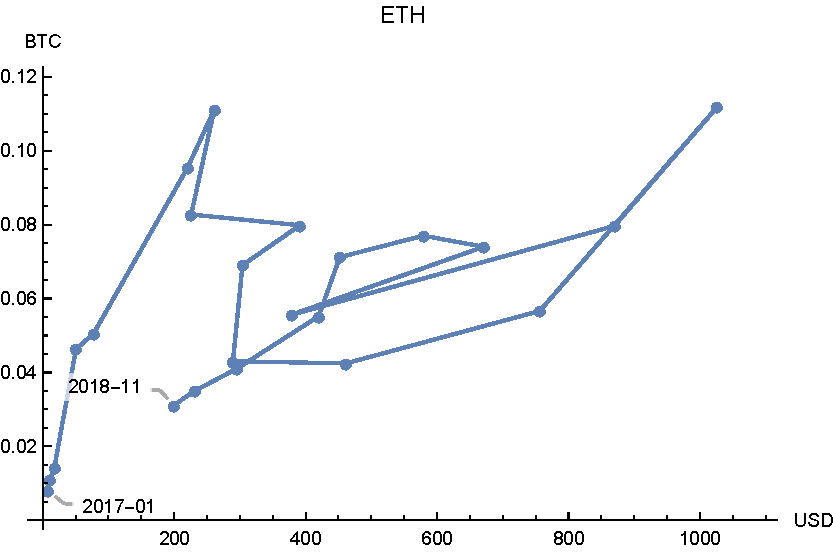
\includegraphics[width=0.45\textwidth]{figures/eth.pdf}\label{fig:eth}}
	\hfill
	\subfloat[XRP]{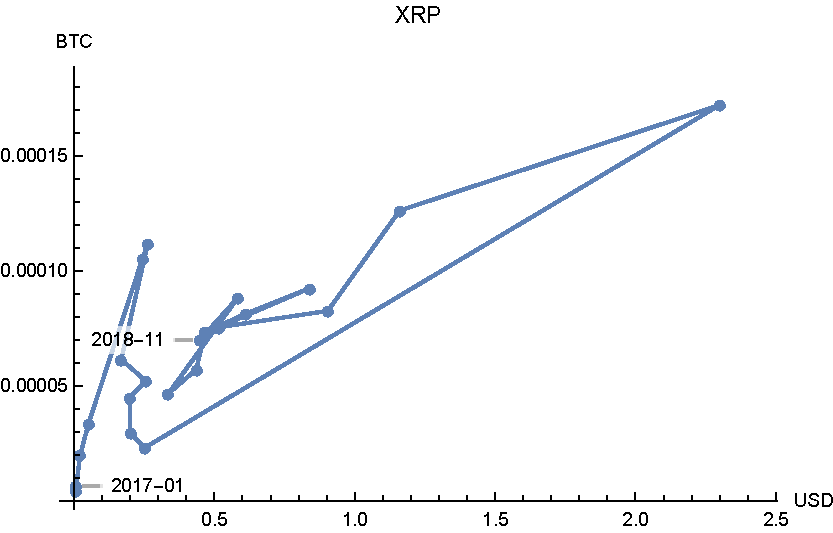
\includegraphics[width=0.45\textwidth]{figures/xrp.pdf}\label{fig:xrp}}
	\caption{Volatility in cryptocurrencies}
	\label{fig:fiatandcrypto}
\end{figure}

We show a connected scatter plot in Figure~\ref{fig:fiatandcrypto} that shows two cryptocurrencies, ETH and XRP (from Ripple) plotted against two reference currencies: the USD on the x-axis as a currency with government-managed stability, and Bitcoin which has no stability mechanism. Like Bitcoin, neither ETH nor XRP have a stability mechanism. The reader might anticipate one of two things: either (i) they move independently from the reference currencies (diagonal movements along the 2/6 direction) or (ii) they move in a way that is correlated to Bitcoin (3/7 movements) because the market prices all cryptocurrencies like a sector. From Figure~\ref{fig:fiatandcrypto}, it is fairly apparent that (i) is correct. The graph displays XRP's strong price surge in December 2017.


\begin{figure*}[t]
	\centering
	\subfloat[CAD]{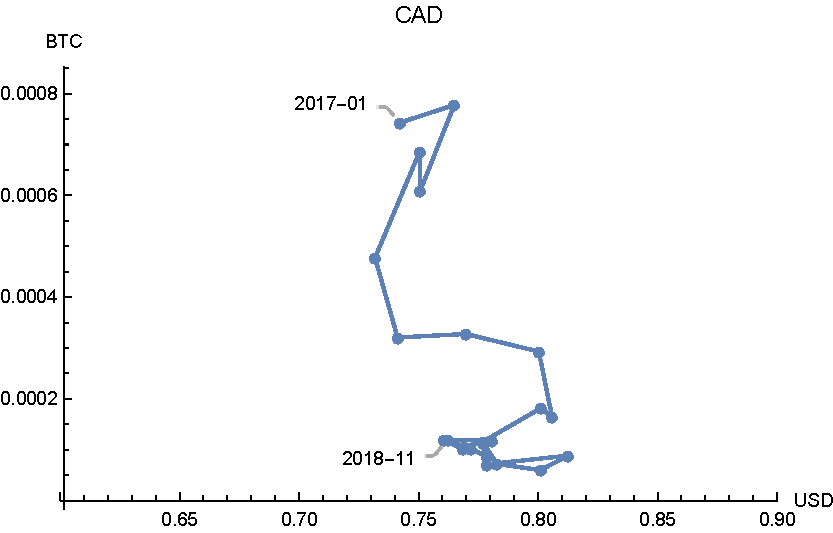
\includegraphics[width=0.45\textwidth]{figures/cad.pdf}\label{fig:cad}}
	\hfill
	\subfloat[EUR]{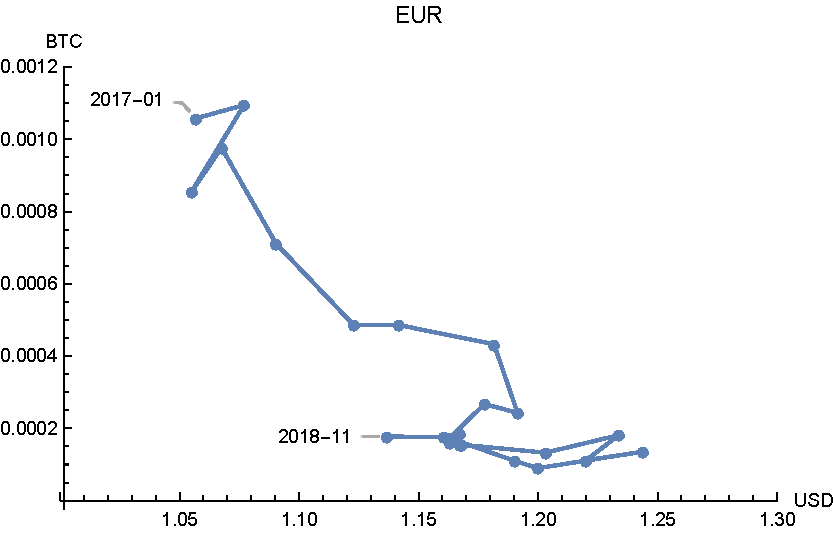
\includegraphics[width=0.45\textwidth]{figures/eur.pdf}\label{fig:eur}}
	\hfill
	\subfloat[Tether]{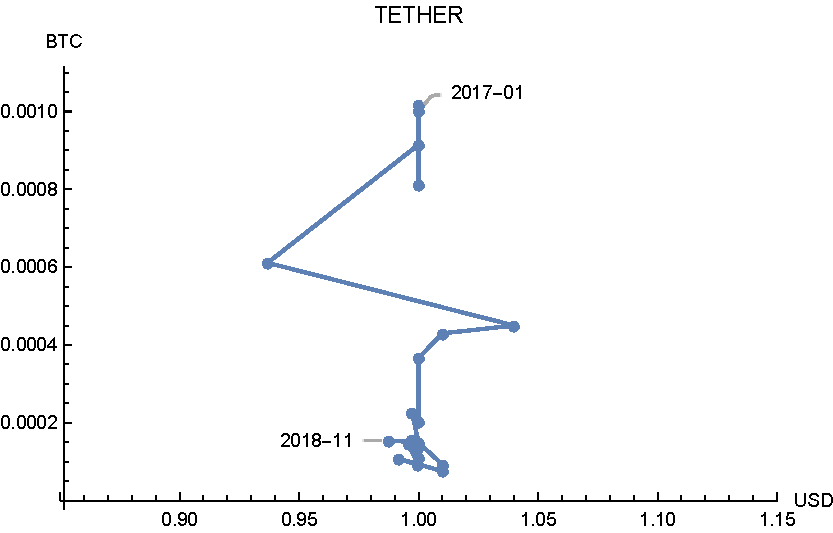
\includegraphics[width=0.45\textwidth]{figures/tether.pdf}\label{fig:tether}}
	\hfill
	\subfloat[BitUSD]{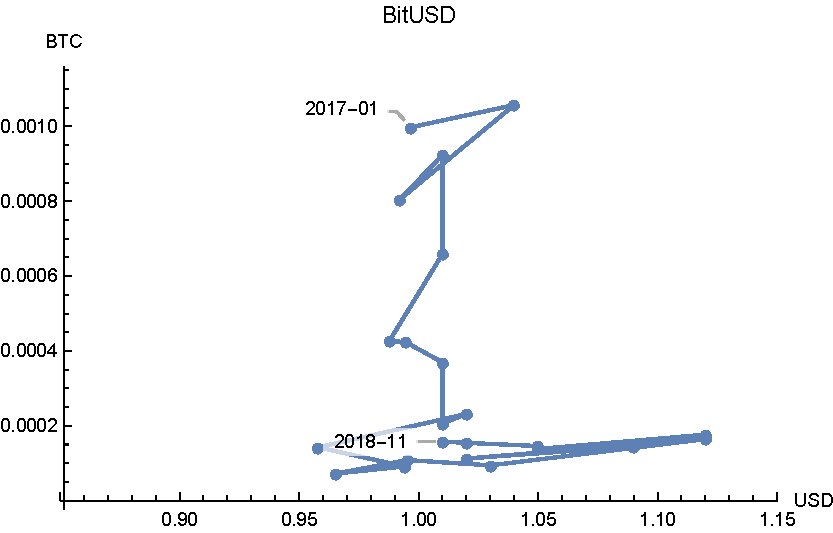
\includegraphics[width=0.45\textwidth]{figures/bitusd.pdf}\label{fig:bitusd}}
	\caption{Stability in two government-issued fiat currencies (CAD and EUR) and two stablecoin projects (Tether and BitUSD). Note that the x-axis is sized consistently across all four plots, with a \$0.30 USD spread. }
	\label{fig:all}
\end{figure*}

Next we plot a number of stablecoins in Figure~\ref{fig:all}. The top two plots are governmental currencies, the Canadian dollar and the Euro, which have no formal relationship to the USD but are managed by their central banks using similar policies and have intertwined economies. The bottom two currencies are two stablecoins, Tether (directly backed with USD) and BitUSD (indirectly backed with USD). All four currencies exhibit movements in 1/5 direction which indicate that most price movements are due to Bitcoin's volatility and not the volatility of either the plotted currency or USD. Note also that the spread of the x-axis is consistent across all four plots to allow cross-comparison. Both Tether and BitUSD exhibit some volatility. When Tether breaks from its stability with the USD, it moves in diagonal movements that are not correlated with either Bitcoin or USD. When BitUSD loses its stability relative to the USD, it moves in a horizontal 3/7 direction which is correlated with BTC.

%========================%

\subsection {Ethereum's gas: a stable `coin'?}\label{sec:GasInvs}

\begin{figure}[t]
	\centering
	\subfloat[Ethereum gas with respect to ETH and USD.]{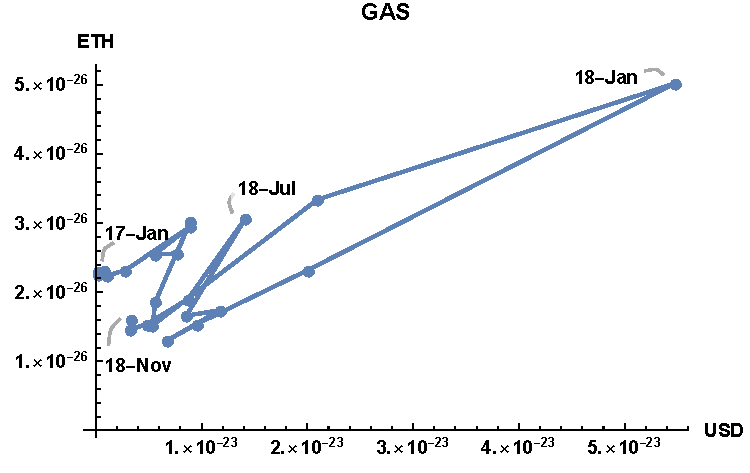
\includegraphics[width=0.45\textwidth]{figures/gasetherusd.pdf}\label{fig:gasetherusd}}
	\hfill
	\subfloat[Ethereum gas with respect to ETH and Electricity.]{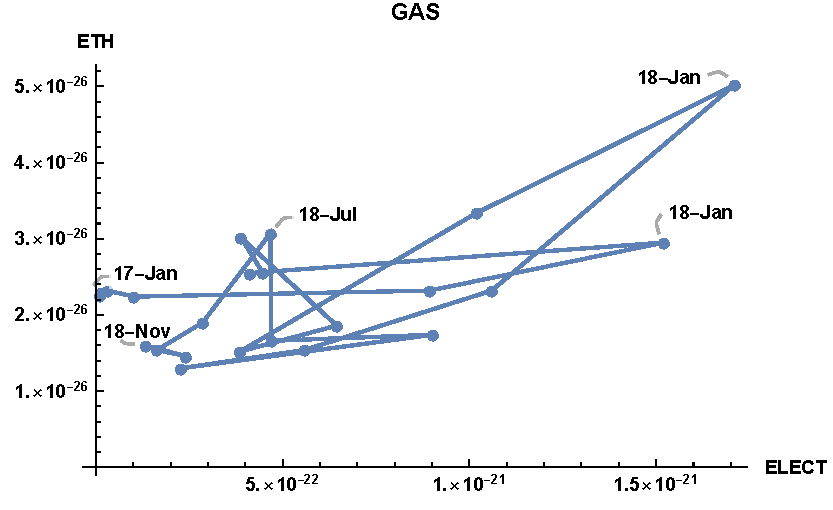
\includegraphics[width=0.49\textwidth]{figures/gaselectricityether.pdf}\label{fig:gaselectricityether}}
	\caption {Ethereum average gas price variations with respect to Ether, USD, and Electricity. As mentioned in the Section~\ref{sec:GasInvs}, the drastic movement in the chart represents a specific event. Data is from January 2017 to November 2018.}
	\label{fig:gas}
\end{figure}

DApps on Ethereum execute arbitrary code provided by the owner of the DApp. While this code might be written in a high-level programming language like Solidity, it is compiled to a compact representation (called `bytecode') that is a set of low-level instructions to the environment (Ethereum virtual machine or EVM). Because different functions will have different complexities, the user running the function pays in proportion to the number of instructions, the complexity of the instructions, and the storage requirements. This means that each operation has a fixed price. Naturally the operations might be priced in ETH, since this the on-board currency, however this would cause the price of computation to be as volatile as Ether itself. Instead, Ethereum uses a pseudo-currency called gas.\footnote{http://ethdocs.org/en/latest/contracts-and-transactions/account-types-gas-and-transactions.html\#what-is-gas} Each instructions has a fixed price in gas. A user who wants to run a function will offer to pay a certain amount of ETH per unit of gas to the miner who finalizes the function. Miners will generally choose which functions to run first based on how much ETH/gas they offer, and they might ignore functions that offer too little ETH/gas. We describe gas as a pseudo-currency because it cannot be directly stored or transacted, however we will revisit this below.

Gas was envisioned as maintaining a relatively stable value where a particular function should cost the same amount (say in USD) over time, even as the price of ETH changes dramatically (as seen in Figure~\ref{fig:eth}). We first investigate how successful gas has been with the charts in Figure~\ref{fig:gas}, which show the monthly average gas price variations with respect to USD and ETH in the first chart; and electricity and USD in the other. Electricity data is from a US-based average index which does not necessarily reflect the costs of mining on a global blockchain, like Ethereum, but if gas were correlated to electricity generally, it should be evident from a representative energy index. Gas demonstrates diagonal movements along the 2/6 direction meaning that it actually moves independently of ETH, USD and electricity. There is no strong evidence of stability. This could be due to a few factors. First, the graph is dominated by one large spike and one moderate spike which correspond to (i) when the popular Ethereum game Cryptokitties \footnote{Cryptokitties website \url{https://www.cryptokitties.co/}} was first launched (January 2018) and, (ii) when the China-based crypto exchange FCOIN \footnote{Fcoin website \url{https://www.fcoin.com}} was launched (July 2018) and required a lot of on-chain voting. Both these events  clogged up the Ethereum network and increased the gas price as users had to pay more gas for their transactions to go through. Second, it is probably true that users do not have a strong mental model of how much gas to stake for a computation and rely heavily on the user interface for prompts about gas.

Although gas might become a stable unit of account, it is not a store of value because it cannot be held or transacted. However gas could be used to back a stablecoin, much like the coins in the directly-backed category. Amazingly, such a gas-backed coin could even be made redeemable.Ethereum is designed in such a way that it allows users to create a smart contract which stockpile and swaps gas with other tokens. Operations that store data on Ethereum blockchain modify its global state hence they are very expensive. So in order to incentivize users to free up space on the blockchain, Ethereum refunds the amount of gas users paid if they delete their smart contracts or stored data~\cite{wood2014ethereum}. GasToken is a directly-backed and redeemable tokenization of gas.\footnote{https://github.com/projectchicago/gastoken} When the gas price is low (\eg 1 Gwei), users can store some data on the GasToken contract and create GasTokens. Later when the gas price increases (\eg 50 Gwei), users can redeem their GasTokens. However they do not receive ETH back; rather, they use the tokens to pay the transaction fees for other computations. 

As users' mental model of gas improves over time, the volatility of gas has the potential to reduce. Gas-backed tokens represent a new class of stablecoin that float in value without any direct ties to USD, references to exchange rates, or explicit intervention mechanisms. It is an interesting subject worthy of further research. 

%========================%

%\subsection{Consequences for Central Banking}

%Interest rates: borrower pays her loan + interest
%Negative interest rate: borrower is paid the interest + she uses the loan
%Sweden and Japan are examples of countries that use NIR

%========================%

%\subsection{Liquidity Crisis and others}


%========================%

\section{Conclusion}

In this paper, we provide a survey of active stablecoin projects. Unlike previous research studies performed on this topic, we selectively use the concepts from finance while eliminating the jargons. In addition, rather than focusing on the details of how particular `brands' of stablecoins work, we thoroughly describe the fundamental mechanics and concepts to achieve price stability. Respectively, we show the taxonomy we use to classify stablecoins which represents the techniques to build a stablecoin. Additionally, we evaluate different price stability achieving mechanics based on their fundamental design decisions and trust models. The comparative evaluation framework highlights the advantages and disadvantages of each techniques more precisely. Eventually, we explore the potential stable index-cryptocurrencies (namely Ethereum gas) in the context of stablecoins.







%==========================================%
